\documentclass[a4paper,12pt]{report}
\usepackage[utf8x]{inputenc}
\usepackage[brazil]{babel}
\usepackage[T1]{fontenc}
\usepackage{epstopdf}
\usepackage{hyperref}
%\DeclareGraphicsRule{.tif}{png}{.png}{`convert #1 `dirname #1`/`basename #1 .tif`.png}
\usepackage{tikz}
\usepackage{indentfirst}
\hyphenation{li-vro tes-te cha-ve bi-blio-te-ca}
\hyphenation{co-men-t-rio re-fe-rn-cia}
\usetikzlibrary{positioning,shapes,shadows,arrows}
\newcommand{\HRule}{\rule{\linewidth}{0.5mm}}
\usepackage{setspace}
\usepackage{enumitem}
\usepackage{listings}
\usepackage{color}
\usepackage{makecell}
\usepackage{float}

\linespread{1.3}
\pagestyle{plain}

\usepackage{color}
\definecolor{lightgray}{rgb}{.9,.9,.9}
\definecolor{darkgray}{rgb}{.4,.4,.4}
\definecolor{purple}{rgb}{0.65, 0.12, 0.82}
\lstdefinelanguage{JavaScript}{
  keywords={break, case, catch, continue, debugger, default, delete, do, else, false, finally, for, function, if, in, instanceof, let, new, null, return, static, switch, this, throw, true, try, typeof, var, void, while, with},
  morecomment=[l]{//},
  morecomment=[s]{/*}{*/},
  morestring=[b]',
  morestring=[b]",
  ndkeywords={class, export, boolean, throw, implements, import, this},
  keywordstyle=\color{blue}\bfseries,
  ndkeywordstyle=\color{darkgray}\bfseries,
  identifierstyle=\color{black},
  commentstyle=\color{purple}\ttfamily,
  stringstyle=\color{red}\ttfamily,
  sensitive=true
}
\lstset{
   language=JavaScript,
   backgroundcolor=\color{lightgray},
   extendedchars=true,
   basicstyle=\footnotesize\ttfamily,
   showstringspaces=false,
   showspaces=false,
   numbers=left,
   numberstyle=\footnotesize,
   numbersep=9pt,
   tabsize=2,
   breaklines=true,
   showtabs=false,
   captionpos=b
}


\begin{document}

%%%%%%%%%%%%%%%%%%%
% parte frontal
%%%%%%%%%%%%%%%%%%%

\begin{titlepage}

\begin{center}


\includegraphics[width=0.20\textwidth]{./logo.jpeg}\\[0.8cm]

\textsc{\LARGE Universidade Federal do Rio de Janeiro}\\
\textsc{Departamento de Ciência da Computação}\\[0.0cm]


% Title
\HRule \\[0.4cm]
{ \huge \bfseries Avaliação e Desempenho }\\[0.4cm]
{ \large \bfseries Simulador de Filas com Prioridade } \\[0.4cm]
\small Professor \emph{Paulo Aguiar}\\
\HRule \\[0.6cm]


% Author and supervisor
\begin{minipage}{0.6\textwidth}
  \begin{flushleft} 
  \emph{Componentes:}\\
  Eduardo Costa \\
  Guilherme Herzog \\
  Lucas Carneiro
  \end{flushleft}
\end{minipage}
\begin{minipage}{0.3\textwidth}
  \begin{flushright}
  \emph{DRE:} \\
  112226744 \\
  112182932 \\
  112205251
  \end{flushright}
\end{minipage}

\vfill

\vspace{25pt}

\begin{minipage}{1.0\textwidth}
  \small A implementação inicial do simulador foi escrita em papel por todos juntos, mas em muitas partes as tarefas foram divididas. \emph{Eduardo} foi essencial na implementação do cálculo das médias e intervalo de confiança de todas as métricas. \emph{Guilherme} foi responsável pela interatividade, interface, gráficos, tabelas e pela implementação do RNG. \emph{Lucas} foi responsável por transformar o rascunho do simulador em código e verificar a corretude do mesmo. Todos participaram igualmente no trabalho.
  
\end{minipage}

\begin{minipage}{1.0\textwidth}

\end{minipage}

\vfill


% Bottom of the page
{\large \today}

\end{center}

\end{titlepage}

%\begin{abstract}
%\end{abstract}

%\begin{samepage}
\begin{spacing}{1.25}
\chapter*{Siglas}
\begin{list}{$\bullet$}{}
  \item[VA] - Variável Aleatória.
  \item[IC] - Intervalo de Confiança.
  \item[$N_{q1}$] - Número de pessoas em espera na fila 1.
  \item[$N_{q2}$] - Número de pessoas em espera na fila 2.
  \item[$N_{s1}$] - Número de pessoas em execução na fila 1.
  \item[$N_{s2}$] - Número de pessoas em execução na fila 2.
  \item[$N_1$] - Número de pessoas na fila 1 (espera + execução).
  \item[$N_2$] - Número de pessoas na fila 2 (espera + execução).
  \item[$W_1$] - Tempo de espera da fila 1.
  \item[$W_2$] - Tempo de espera da fila 2.
  \item[$X_1$] - Tempo do primeiro serviço.
  \item[$X_2$] - Tempo do segundo serviço.
  \item[$T_1$] - Tempo total de execução da fila 1.
  \item[$T_2$] - Tempo total de execução da fila 2.
  \item[$\rho$] - Taxa de utilização total do sistema = 2$\lambda$.
  \item[$\lambda$] - Taxa de entrada do sistema.
  \item[$\mu$] - Taxa de serviço do sistema.
  
\end{list}
\end{spacing}
%\end{samepage}

\tableofcontents

% Lista de Figuras
% \listoffigures

% Lista de Tabelas
% \listoftables


\setlength{\parskip}{\baselineskip}%
% espaçamento vertical entre parágrafos

%%%%%%%%%%%%%
% Introdução
%%%%%%%%%%%%%
\chapter{Introdução}

\section{O Simulador}

O simulador pode ser acessado no link \url{https://guiherzog.github.io/simulador-ad-web/} ou baixado e executado localmente na máquina, no repositório \url{https://github.com/guiherzog/trab-ad-2017.2}.

\begin{figure}[H]
\centering
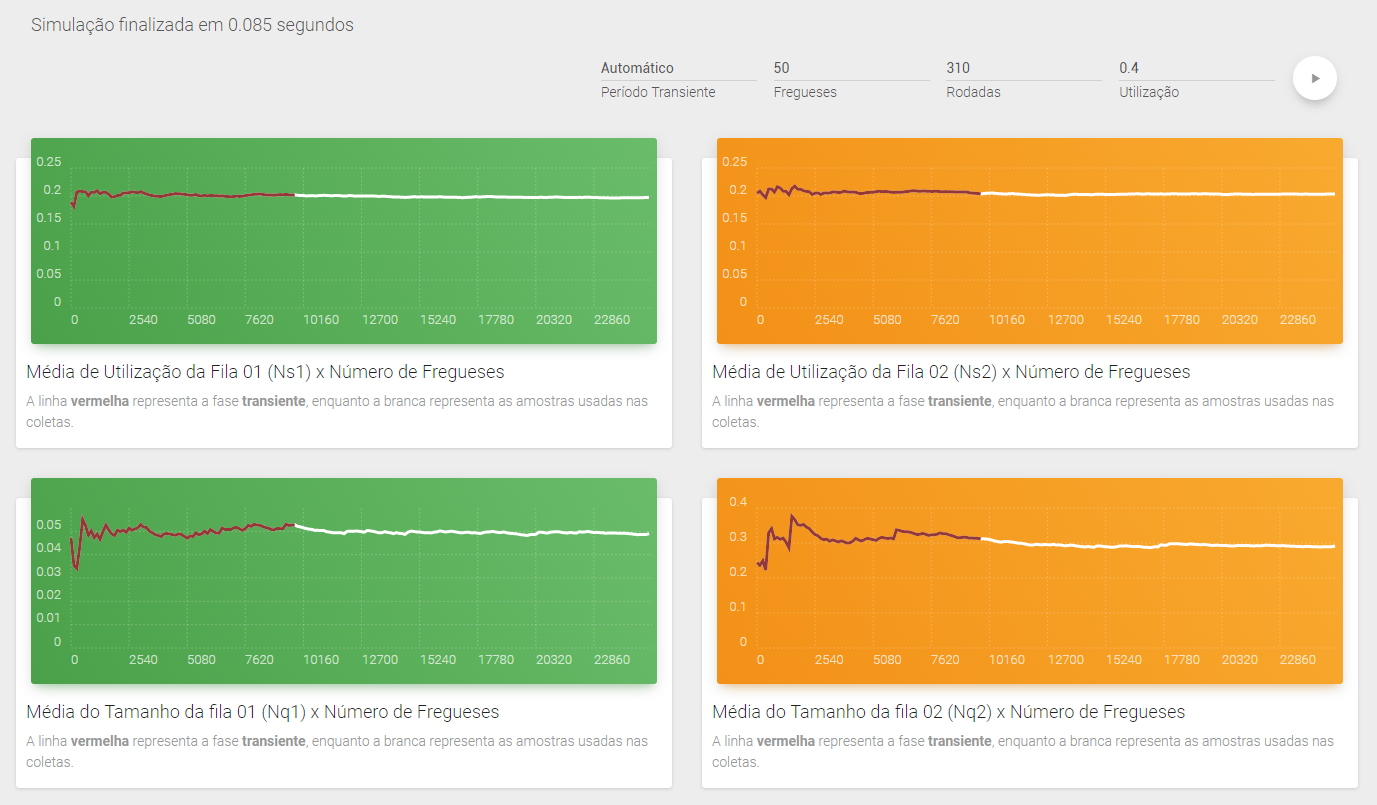
\includegraphics[width=0.7\textwidth]{./graficos/overview.png}
\vspace{-3mm}
\caption{Visão Geral do Simulador}
\label{fig:overview}
\end{figure}

\subsection{Descrição de Requisitos}

Neste trabalho, foi desenvolvido um simulador de um sistema no qual duas filas disputam um servidor, e uma delas tem prioridade preemptiva sobre a outra.

A fila 1 tem chegadas segundo um processo Poisson com taxa $\lambda$. Após o primeiro serviço, os fregueses vão para a fila 2, com menos prioridade, onde serão servidos pela segunda vez. Depois desse segundo serviço, vão embora. Não chegam fregueses na fila 2. A fila 1 tem prioridade sobre a fila 2, de modo que um serviço em andamento na fila 2 pode ser interrompido por uma chegada na fila 1. As filas operam no modo FCFS (\emph{First Come First Served}).

\subsection{Implementação}

Para simularmos o funcionamento da fila em código de maneira similar a realidade, utilizamos um loop, que continua executando enquanto o número de pessoas que deixaram o sistema (caracterizado pela saída da fila 2) for menor do que o número total de pessoas configurado como parâmetro inicial, que é definido pelo $n\acute{u}mero \ de \ fregueses \ por \ rodada \times n\acute{u}mero \ de \ rodadas$. A iteração desta repetição não é feita por unidades de tempo, mas por períodos de tempo, iguais à taxa de chegada de fregueses no sistema. Por conta disso, cada iteração do loop acontece no momento de chegada de um novo freguês no sistema. Esta chegada é, por padrão, gerada aleatoriamente utilizando uma taxa exponencial, mas também pode funcionar por meio determinístico (utilizado para testes de corretude), junto com a geração do tempo de execução de cada freguês.

Dentro de cada iteração, primeiramente é calculado o tempo que se passou desde a última chegada. Após obter este valor, o mesmo é usado para seguir com o fluxo do sistema, diminuindo o tempo de execução restante do freguês que se encontra dentro do servidor, e, no caso do seu tempo restante ser menor do que o tempo calculado desde a última chegada, reduzir o tempo restante de execução do próximo freguês, e assim sucessivamente. Isso se repete até o momento em que todo o tempo calculado tiver sido usado para atender os fregueses que se encontravam nas filas, ou até ambas as filas estarem vazias. Apesar de termos implementado uma fila de eventos que poderia ser utilizada para controlar esta ordem, todo o controle da ordem de execução do sistema é feito por conta da própria estrutura de dados de cada fila, que adiciona novos fregueses em seu primeiro índice vazio, ao final da fila. A fila de eventos acabou sendo usada apenas como uma maneira de testar a execução do simulador e verificar a correção, por meio da análise de sua ordem em casos pequenos.

Durante o processo da simulação, também é feito o controle de cada rodada, de maneira com que os resultados de cada uma delas seja preservado separadamente. Para a separação entre rodadas e obtenção de resultados, foi utilizado o método \emph{batch}. Neste método, são desprezados os fregueses de um período inicial, denominado \textbf{fase transiente}, em que o sistema ainda não entrou em equilíbrio. Após o equilíbrio ser atingido, os dados passam a ser coletados, tomando cuidado para que métricas de fregueses de diferentes rodadas não sejam misturadas, por meio do conceito de cores (explicado mais a frente). Apenas no início da simulação haverá dados descartados, pois serão a fase transiente para a primeira rodada. Para as rodadas seguintes, isto não será necessário no método \emph{batch}, pois o sistema se mantém em equilíbrio.

\section{Ferramentas de Desenvolvimento}

\subsection{Ambiente Utilizado}
Para o desenvolvimento do simulador foi utilizado o framework \textbf{NodeJS}, que funciona através da linguagem \emph{JavaScript}. Desta forma, o simulador pode ser executado em qualquer máquina, independente de sistema operacional. Além disso, pela experiência do grupo utilizando esta plataforma, foi possível criar uma interface visual moderna e eficiente para a visualização das métricas de cada fila. Para a execução do simulador, foram criados arquivos executáveis para Windows e Linux, e foi feita também uma versão Web.

Cada integrante do grupo usou uma máquina e sistema operacional diferente para a realização dos testes, sendo estes:
\vspace{-1.5em}
\begin{itemize}
	\item Windows 10, Processador Core i7 e 32GB de RAM.
    \item Fedora 25 (Linux), Processador Core i7 3770 e 8GB de RAM.
    \item MacOS High Sierra, Processador Core i7 e 8GB de RAM.
\end{itemize}

No entanto, para efeito de comparação, todos os gráficos e tempos exibidos no relatório foram rodados na primeira máquina (Windows 10).

Centenas de experimentos foram executados na simulação com diversos parâmetros. Para efeitos de observação da complexidade e eficiência do simulador, foram executados testes variando o número de fregueses e fixando os outros parâmetros, de acordo com a tabela abaixo:

\begin{center}
\begin{tabular}{ c c }
  \hline
  \textbf{Parâmetro} & \textbf{Valor}\\
  \hline
  $\rho$ ($\rho_1 + \rho_2$) & 0,1\\
  Fase transiente & 0\\
  Nº de rodadas & 1\\
  Nº de fregueses & variável\\
  \hline
\end{tabular}
\end{center}

Após testes com diferentes números de fregueses, sempre dobrando, pudemos observar o comportamento do crescimento do tempo de execução. Os resultados obtidos foram os seguintes:

\begin{center}
\begin{tabular}{c c}
\hline
\textbf{Fregueses} & \textbf{Tempo} \\[-4pt]
\textbf{($\times$1000)} & \textbf{(segundos)}\\[3pt]
\hline
10 & 0,03\\
20 & 0,04\\
40 & 0,07\\
80 & 0,15\\
160 & 0,30\\
320 & 0,59\\
640 & 1,18\\
\hline
\end{tabular} \qquad \qquad
\begin{tabular}{c c}
\hline
\textbf{Fregueses} & \textbf{Tempo} \\[-4pt]
\textbf{($\times$1000)} & \textbf{(segundos)}\\[3pt]
\hline
1280 & 2,28\\
2560 & 4,88\\
5120 & 9,67\\
10240 & 19,45\\
20480 & 40,12\\
40960 & 78,97\\
61440 & 110,43\\
\hline
\end{tabular}
\end{center}


Neste experimentos o número de fregueses dobrou a cada rodada e os tempos de execução foram coletados e salvos numa planilha. É interessante notar que plotando os dados dessa tabela em um gráfico, foi possível perceber que a complexidade de tempo do simulador é linear (\textbf{O(n)}) em função do número total de fregueses executados, como pode ser visto no gráfico abaixo.


\begin{figure}[H]
\centering
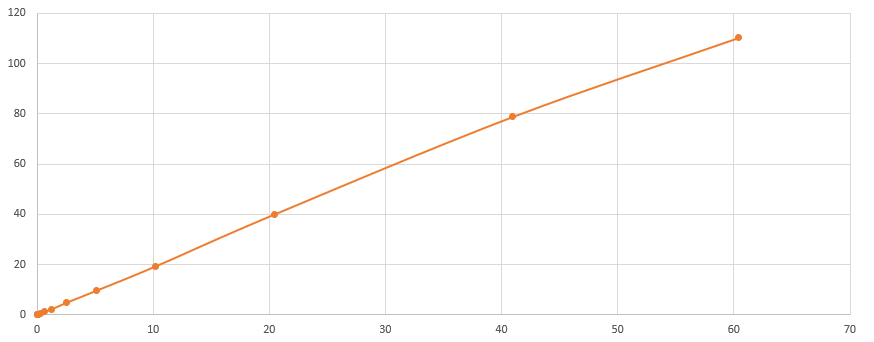
\includegraphics[width=1\textwidth]{./graficos/tempoexecucao2.png}
\vspace{-10mm}
\caption{Tempo de execução (segundos) $\times$ Total de fregueses (em milhões)}
\label{fig:tempo_execucao}
\end{figure}


Testes similares foram feitos com outros valores de $\rho$, e os tempos de execução foram similares e não variavam mais do que 10\%. 

Apesar do simulador calcular as médias incrementalmente para diminuir o tempo de execução, ainda é necessário armazenar todas elas para plotar as tabelas e os gráficos. Por isso, por razões de limitações de espaço de memória, não foi possível armazenar dados de mais de 70 milhões de fregueses, pois isto ocuparia mais de 4GB de memória, o que não é suportado pelo \emph{framework} usado. Desta forma, este é o limite total de fregueses por execução. Porém, este limite não prejudicou a coleta e análise dos resultados, pois o total de fregueses utilizado nos testes ($n\acute{u}mero \ de \ fregueses \ por \ rodada \times n\acute{u}mero \ de \ rodadas + fase \ transiente$) foi bastante inferior a este limite.

\subsection{Tecnologias Gráficas e Interativas}

As ferramentas gráficas e interativas foram essenciais na fase de otimização dos parâmetros da simulação e para a visualização dos resultados. Diversas tecnologias foram aplicadas para possibilitar a criação dessas funcionalidades. Para renderização dos gráficos foi utilizada a biblioteca \emph{Chartist.js}, para a criação da interface foi utilizada a biblioteca \emph{Bootstrap} e \emph{jQuery}. Além disso, foi utilizado o framework \emph{Electron}, que torna possível o acesso a recursos de baixo nível por aplicações web, como \emph{threads} e bibliotecas de alta performance. O design foi desenvolvido com o auxílio de um template chamado \emph{Material Dashboard}.

\subsection{Organização da Equipe}

Para se organizar durante o desenvolvimento do projeto, foi utilizado um sistema de controle de versionamento de código conhecido como \textbf{Git}. Além disso, para escrever o relatório foi usada a ferramenta \textbf{ShareLaTeX}, uma aplicação web que permite que diversos colaboradores escrevam documentos em \textbf{LaTeX} simultaneamente. Foram também usadas algumas ferramentas para controle das tarefas pendentes de cada integrante.

\section{Estruturas Internas}

Nesta seção serão discutidas as estruturas internas principais do simulador, assim como suas características, vantagens e limitações.

\subsection{Eventos}
Neste simulador, os eventos são objetos do tipo \emph{Event}, e possuem as seguintes propriedades:
\begin{enumerate}
	\itemsep1em
	\item \textbf{Tempo}: representa o instante do tempo do sistema em que o evento ocorre.
    \item \textbf{ID do freguês}: identificador do freguês no sistema.
    \item \textbf{Tipo}: o tipo do evento, que pode ser ``chegada no sistema'' ou ``fim de serviço''.
    \item \textbf{Prioridade}: número que representa a prioridade do evento. Quanto menor o número, mais prioridade. Neste simulador, terá apenas os valores ``1'' ou ``2'', indicando a fila 1 ou 2, respectivamente.
\end{enumerate}

Os eventos são guardados num vetor. Conforme são processados, são removidos. O vetor sempre guarda a quantidade mínima necessária de eventos: apenas os que ainda não foram processados. Entretanto, os mesmos não são utilizados para o funcionamento da simulação, apenas para o teste de correção da simulação. 

\subsection{Fregueses}
Os fregueses são objetos do tipo \emph{Customer}, e possuem as seguintes propriedades:
\begin{enumerate}
	\itemsep1em
	\item \textbf{Identificador}: número que identifica o freguês no sistema.
    \item \textbf{Tempo de chegada na fila 1}: momento em que o freguês chega no sistema e começa a esperar na fila 1
    \item \textbf{Tempo de chegada na fila 2}: momento em que o freguês termina a execução do serviço 1 e começa a esperar na fila 2
    \item \textbf{Duração do serviço 1}: tempo de duração do serviço 1
    \item \textbf{Duração do serviço 2}: tempo de duração do serviço 2
    \item \textbf{Tempo de serviço restante}: tempo de serviço que ainda falta ser executado. Útil para saber o tempo restante quando o freguês é interrompido em sua execução do serviço 2.
    \item \textbf{Prioridade}: número que representa a prioridade da fila onde o freguês está no momento, ou o número de seu serviço sendo executado. Quanto menor o número, mais prioridade. Neste simulador, terá apenas os valores ``1'' ou ``2'', indicando fila/serviço 1 ou 2, respectivamente.
\end{enumerate}

\subsection{Métricas}

Todas as métricas obtidas da simulação são armazenadas em um hashmap, separadamente por rodada. Durante a simulação, cada rodada tem suas métricas incrementadas conforme novos fregueses chegam, executam e saem do sistema. Ao final da execução da simulação, as métricas são transformadas em médias para cada rodada, e também como média geral. Além disso, estados temporários de cada métrica são utilizados para construir os gráficos exibidos na interface gráfica do programa, e calcular variâncias.

\section{Geração de Variáveis Aleatórias}
O gerador de números aleatórios padrão do \emph{JavaScript} não permite a utilização de semente e não é confiável para geração de números ``verdadeiramente'' aleatórios. Em muitas aplicações, as funções padrões são suficientes. Porém, na simulação, era necessário garantir a aleatoriedade e independência entre os valores gerados, além de permitir que o experimento seja replicado. Por isso, utilizamos a biblioteca \emph{seedrandom} para que fosse possível gerar números aleatórios a partir de uma semente específica e com uma maior garantia da aleatoriedade. Para mais detalhes, é possível consultar a documentação da biblioteca neste link: \url{https://github.com/davidbau/seedrandom}.

A partir de um número aleatório com distribuição uniforme, é possível gerar um número aleatório com distribuição exponencial. Seja $rand$ um número aleatório entre 0 e 1 com distribuição uniforme. A partir da expressão abaixo, será gerado um número aleatório com distribuição exponencial com taxa $\lambda$:
\[ - \ln \frac{1 - rand}{\lambda}  \]


Através do código abaixo, localizado no arquivo \emph{Utils.js}, a semente pode ser definida:

\begin{lstlisting}
    const randomSeed = seedrandom('semente');
\end{lstlisting}

Como \emph{seedrandom} retorna uma função, a variável \emph{randomSeed} será uma função, e cada vez que for chamada gerará o próximo número da sequência.

Definida a semente, o método \emph{getRandomExp} pode ser chamado, com a taxa como parâmetro, para a geração dos números aleatórios com distribuição exponencial:

\begin{lstlisting}
    static getRandomExp(rate){
        return - Math.log(1 - randomSeed()) / rate;
    }
\end{lstlisting}


\section{Conceito de Cores}

Por conta do uso do método \emph{batch} para separação de rodadas, foi necessário utilizar o conceito de cores para garantir que cada freguês tivesse seus valores utilizados apenas no cálculo das métricas da sua rodada. Isso foi conseguido usando o identificador do próprio objeto \emph{Customer}. Dividindo seu valor pelo número de fregueses esperado por rodada, é possível saber qual é a rodada o freguês em questão pertence. Este comportamento é visto abaixo, em um trecho de código que utiliza esta verificação.

\begin{lstlisting}
	executingCustomerRound = Math.floor(executingCustomer.id / nCustomers);
\end{lstlisting}

%%%%%%%%%%%%%
% Testes
%%%%%%%%%%%%%
\chapter{Testes de Correção}
Para garantir o pleno funcionamento do simulador, foram feitos testes com filas D/D/1. Com filas e serviços determinísticos, foi possível ver se os resultados obtidos eram de fato os esperados.

Foi implementado um modo determinístico no simulador, que pode ser ativado através da variável \emph{deterministic}, do tipo booleano. Quando seu valor é \emph{true}, o simulador roda em modo determinístico.
Através do método \emph{setDeterministicArrivals}, é passado para o simulador uma lista de valores a serem gerados para os tempos entre chegadas. Com o modo determinístico ativado, os valores gerados para os tempos entre chegadas não mais serão aleatórios, mas serão pegos na ordem desta lista.

Por exemplo: definindo a lista de chegadas determinísticas como [1,2,4], a primeira chegada ocorrerá no tempo 1, a segunda no tempo 3 (dois segundos após a primeira), e a terceira no tempo 7 (quatro segundos após a segunda).

Similarmente, os métodos \emph{setDeterministicX1s} e \emph{setDeterministicX2s} são usados para definir os tempos determinísticos dos serviços 1 e 2, respectivamente.

A definição da variável e a chamada dos métodos mencionados estão localizados no arquivo \emph{QueueSystem.js}, dentro da função \emph{runRounds}. Como exemplo, abaixo é mostrado o trecho de código para rodar um dos testes determinísticos:

\begin{lstlisting}
	// Usar valores deterministicos no lugar dos gerados aleatoriamente
	let deterministic = true;

	// Definindo valores deterministicos
	Utils.setDeterministicArrivals([1, 2]);
	Utils.setDeterministicX1s([1, 10]);
	Utils.setDeterministicX2s([3, 2]);
\end{lstlisting}


\section{Testes Realizados}

Para testar o simulador, foram feitos alguns testes em cenários simplificados, a fim de verificar que o funcionamento do simulador estava correto. Estes testes estão detalhados a seguir.


\subsection{Teste 1: Apenas Um Freguês}
Neste primeiro teste, foi testada a situação mais simples possível: apenas um freguês chega no sistema, é servido, e vai embora. Para isso, foram utilizadas as seguintes listas de tempos determinísticos:

\vspace{-1.5em}
\begin{itemize}
	\itemsep0pt
	\item Tempos entre chegadas: [1]
    \item Tempos do serviço 1: [3]
    \item Tempos do serviço 2: [4]
\end{itemize}

Dessa forma, o freguês chegará ao sistema no tempo 1, não espera na fila 1, e imediatamente será servido pela primeira vez. Depois, na fila 2, também não espera, e será servido pela segunda vez. Depois, vai embora.

Observando a tabela de resultados do simulador, podemos confirmar que tudo está de acordo com o esperado:


%%%%%%%%%%%%%%%%%%%%%%%%%%%%%%%%%%%
% Comentado
%%%%%%%%%%%%%%%%%%%%%%%%%%%%%%%%%%%
\iffalse
\begin{figure}[h]
\centering
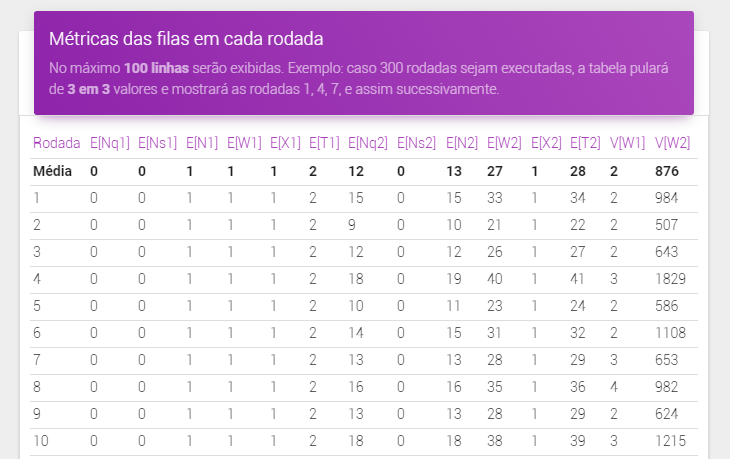
\includegraphics[width=1\textwidth]{./graficos/image_2017-12-10_15-42-42.png}
\caption{Tabela}
\label{fig:asddd}
\end{figure}
\fi
%%%%%%%%%%%%%%%%%%%%%%%%%%%%%%%%%%%
% /Comentado
%%%%%%%%%%%%%%%%%%%%%%%%%%%%%%%%%%%

\begin{center}
\begin{tabular}{ c c c c c c c c c }
  \hline
  \textbf{Rodada} & $N_{q1}$ & $N_{s1}$ & $W_1$ & $X_1$ & $N_{q2}$ & $N_{s2}$ & $W_2$ & $X_2$ \\
  \hline
  1 & 0 & 0 & 0 & 3 & 0 & 0 & 0 & 4 \\
\end{tabular}
\end{center}

Como não há ninguém no sistema no momento que este freguês chega, é esperado que $N_{q1}$, $N_{s1}$, $N_{q2}$ e $N_{s2}$ sejam 0, e o tempo de espera em cada fila também, já que as filas estão vazias. Os únicos valores diferentes de 0 são X1 e X2, como esperado. Portanto, os resultados estão corretos.


\subsection{Teste 2: Dois Fregueses, onde o Segundo Interrompe o Primeiro}
Neste teste, testamos a situação de interrupção. Quando o primeiro freguês está executando o serviço 2, chega o segundo, e o interrompe. Para melhor observar os tempos de cada freguês, foram utilizadas 2 rodadas, com 1 freguês cada. Dessa forma, a tabela com as médias de cada rodada mostrará o valor dos parâmetros de um só freguês. Para este teste, foram utilizadas as seguintes listas de tempos determinísticos:

\vspace{-1.5em}
\begin{itemize}
	\itemsep0pt
	\item Tempos entre chegadas: [1, 2]
    \item Tempos do serviço 1: [1, 10]
    \item Tempos do serviço 2: [3, 2]
\end{itemize}

A tabela de resultados obtida foi a seguinte:
\vspace{-1em}
\begin{center}
\begin{tabular}{ c c c c c c c c c }
  \hline
  \textbf{Rodada} & $N_{q1}$ & $N_{s1}$ & $W_1$ & $X_1$ & $N_{q2}$ & $N_{s2}$ & $W_2$ & $X_2$ \\
  \hline
  1 & 0 & 0 & 0 & 1 & 0 & 0 & 10 & 3 \\
  2 & 0 & 0 & 0 & 10 & 0 & 1 & 2 & 2 \\
  \hline
\end{tabular}
\end{center}

No tempo 1 do sistema o freguês 1 chega, como não há ninguém no sistema seu $N_{q1}$, $N_{s1}$, $N_{q2}$, $N_{s2}$ e $W_1$ são 0. Dois segundos depois, no tempo 3, o freguês 2 chega. Neste momento, o primeiro freguês já terá terminado seu serviço 1 ($N_{q1}$ e $N_{s1}$ do freguês 2 são 0), e estará na execução do serviço 2 há 1 segundo ($N_{s2}$ do freguês 2 é 1). Esta execução do serviço 2 do freguês 1 será interrompida, para que o freguês 2 execute seu serviço 1. Por isso, $W_2$ do freguês 1, que até o momento era 0, terá um acréscimo do tempo do serviço 1 do freguês 2, que é 10. Quando o freguês 2 terminar seu serviço 1, ele irá para o fim da fila 2, e o freguês 1 finalmente poderá continuar seu serviço 2. Como faltavam 2 segundos (já havia executado 1 dos 3 segundos), este tempo será adicionado ao tempo de espera na fila 2 do freguês 2, que será 2. Com isso, vimos que os resultados estão corretos.

\subsection{Teste Maior com Muitos Fregueses}

Neste teste, foram usados os seguinte tempos determinísticos:

\vspace{-1.5em}
\begin{itemize}
	\itemsep0pt
	\item Tempos entre chegadas: [4, 4, 4, 4, 4, 4, 4, 4, 4, 4, ...]
    \item Tempos do serviço 1: [2, 2, 2, 2, 2, 2, 2, 2, 2, 2, ...]
    \item Tempos do serviço 2: [3, 2, 2, 2, 2, 2, 2, 2, 2, 2, ...]
\end{itemize}

O primeiro freguês chegará e terá seu serviço 1 executado. Depois, iniciará o serviço 2, porém, antes de concluir (faltando 1 segundo), o freguês 2 chega. O freguês 2 executará seu primeiro serviço inteiro, e este tempo entrará no W2 do freguês 1. Depois, o freguês 1 terminará o serviço 2, executando o 1 segundo restante. Após isso, o freguês 2 pode finalmente começar seu serviço 2, mas será interrompido quando faltar 1 segundo, pelo freguês 3. Os 2 segundos do serviço 1 do freguês 3 será adicionado ao W2 do freguês 2. Depois, ele executará o que falta do serviço 2, que é 1 segundo. Este comportamento do freguês 2 se repete por todos os outros fregueses.

Sempre que alguém chega, o anterior já terminou o serviço 1. Logo, a média de $N_{q1}$ e $N_{s1}$ de todos os fregueses é 0, e de W1 também. A média de X1 será 2, pois todos têm o mesmo tempo de serviço 1.

Em toda chegada, há apenas 1 freguês no sistema: o freguês anterior. Ele está sempre no servidor, recebendo seu serviço 2. Logo, $N_{q2}$ é 0 para todos os fregueses, e $N_{s2}$ é 1 para todos exceto o primeiro. Com um teste de 10 fregueses, será 0,9.

Para o W2, sabemos que o do primeiro freguês será 2, que é o tempo do serviço 1 do freguês seguinte que o interrompeu. Para todos os fregueses seguintes, será 3, pois, além do tempo 2 do serviço 1 do freguês seguinte, terá que esperar tempo 1 do término do serviço 2 do freguês anterior, que também foi interrompido. Assim sendo, a média de W2 será
\[ \frac{2 + 3 \cdot (n-1)}{n}\]
e a de X2 será
\[ \frac{3 + 2 \cdot (n-1)}{n} \] pois o serviço do primeiro freguês é 3 e o dos outros é 2. Com nosso teste de 10 fregueses, W2 foi 2,7 e X2 será 2,1.


A tabela de resultados do teste neste formato com 10 fregueses está mostrada a seguir:
\vspace{-1em}
\begin{center}
\begin{tabular}{ c c c c c c c c c }
  \hline
  \textbf{Rodada} & $N_{q1}$ & $N_{s1}$ & $W_1$ & $X_1$ & $N_{q2}$ & $N_{s2}$ & $W_2$ & $X_2$ \\
  \hline
  1 & 0 & 0 & 0 & 2 & 0 & 0,9 & 2,7 & 2,1 \\
  \hline
\end{tabular}
\end{center}


\section{Comparação com Dados Analíticos e Conceitos de Filas}

Como curiosidade, e não como forma de garantir a correção dos resultados, será mostrada aqui uma comparação dos intervalos obtidos com os valores reais calculados analiticamente. Foi possível ver que os dados analíticos estavam dentro do intervalo de confiança para todos os parâmetros verificados.

\subsection{Resultados Analíticos}

Foi possível observar que os resultados calculados analiticamente sempre estavam dentro do intervalo de confiança dado pelo simulador, para testes com número de fregueses suficientes.

Como exemplo, mostramos aqui o teste com $\rho$ = 0,4 ($\lambda$ = 0,2). Este $\rho$ representa a taxa de utilização total do sistema, ou seja, $\rho_1$ + $\rho_2$. Os resultados obtidos no simulador, com fase transiente de 15000 fregueses, e 50 rodadas com 5000 fregueses cada, foram os seguintes:

\begin{figure}[H]
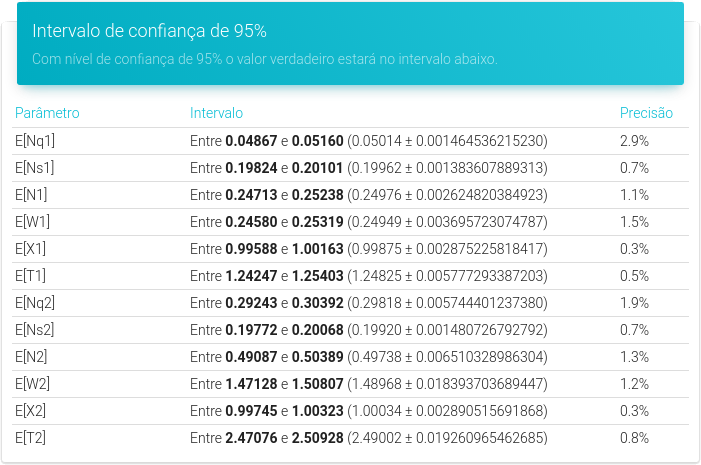
\includegraphics[width=1\textwidth]{./graficos/resultados_simulador_ic.png}
\end{figure}

\vspace{-5mm}

Os resultados obtidos analiticamente foram:
\vspace{-2mm}
\begin{center}
\begin{tabular}{c c}
  \hline
  \textbf{Parâmetro} & \textbf{Valor}\\
  \hline
  $\overline{W_1}$ & 0,25 \\
  $\overline{N_{q1}}$ & 0,05 \\
  $\overline{T_2}$ & 2,5 \\
  $\overline{N_2}$ & 0,5 \\
  $\overline{W_2}$ & 1,5 \\
  $\overline{N_{q2}}$ & 0,3 \\
  \hline
\end{tabular}
\end{center}

Podemos ver que todos os resultados analíticos estão dentro dos intervalos de confiança dados pelo simulador. Além disso, os resultados da simulação mostram que N = $N_{q}$ + $N_{s}$, e T = W + X, comprovando as igualdades conhecidas.

Comparações mais detalhadas serão mostradas mais a frente neste relatório, na seção de resultados.


\subsection{Condições de Estabilidade e Testes Extremos}
Um conceito interessante na Teoria de Filas é a condição de estabilidade. Quando esta condição não é cumprida, a fila crescerá indefinidamente, apresentando algumas características interessantes. Por exemplo, $\overline{N}$ e $\overline{W}$ tenderiam ao infinito conforme fossem chegando pessoas nas filas.

No simulador, esse fenômeno também pode ser observado. Quanto maior o valor de $\rho$, maior ficaram os gráficos das médias de N e W2, além de outros parâmetros. Caso $\rho$ ($\rho_1$ + $\rho_2$) seja muito maior do que 1,0, o tempo de execução cresce indefinidamente, pois nenhum freguês da fila 02 consegue ser executado. Os gráficos abaixo mostram como $\overline{Nq2}$ cresceu conforme $\rho$ foi sendo incrementado para valores acima de 1.

\begin{figure}[H]
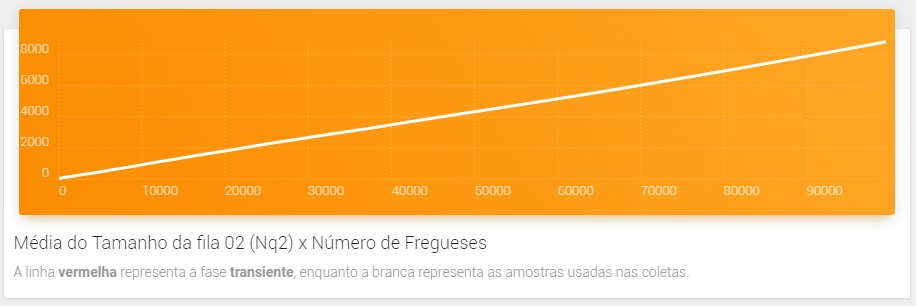
\includegraphics[width=1\textwidth]{./graficos/nq2rho1_1.png}
\vspace{-10mm}
\caption{Simulação com $\rho$ = 1,1 e 100 mil fregueses.}
\end{figure}

\begin{figure}[H]
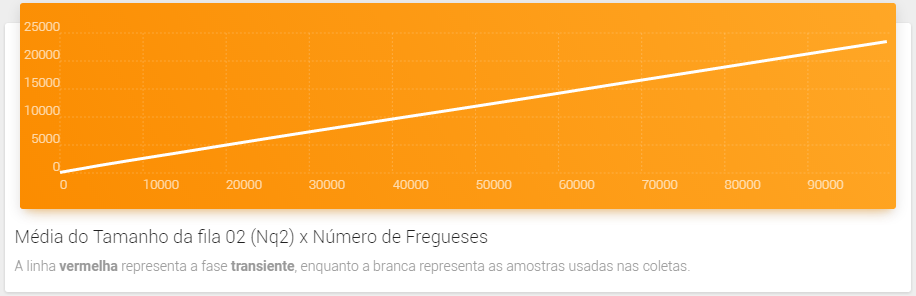
\includegraphics[width=1\textwidth]{./graficos/nq2rho1_3.png}
\vspace{-10mm}
\caption{Simulação com $\rho$ = 1,3 e 100 mil fregueses.}
\end{figure}

%%%%%%%%%%%%%
% Fase transiente
%%%%%%%%%%%%%
\chapter{Estimativa da Fase Transiente}

Nesta seção, será abordado como a fase transiente foi definida e qual a sua influência na qualidade das medidas. Além disso, será dada uma explicação detalhada de seu cálculo no simulador.

\section{Escolha da Fase Transiente}

Para estimar o tamanho necessário para a fase transiente, foram feitos testes com diferentes valores de $\rho$ ($\rho_1$ + $\rho_2$). Para cada valor, a simulação foi rodada dezenas de vezes, a fim de observar os gráficos e notar a partir de que ponto as médias começavam a convergir.

Pelas características do simulador, foi notado que os parâmetros da fila 2 foram os que mais demoravam para entrar em equilíbrio, pois ela pode ser interrompida muitas vezes. Quanto maior o $\rho$, maior a probabilidade disso acontecer. Abaixo é possível observar uma comparação de diferentes gráficos dos parâmetros das filas 1 e 2 utilizando $\rho$ = 0.95 para causar maior instabilidade.

\begin{figure}[H]
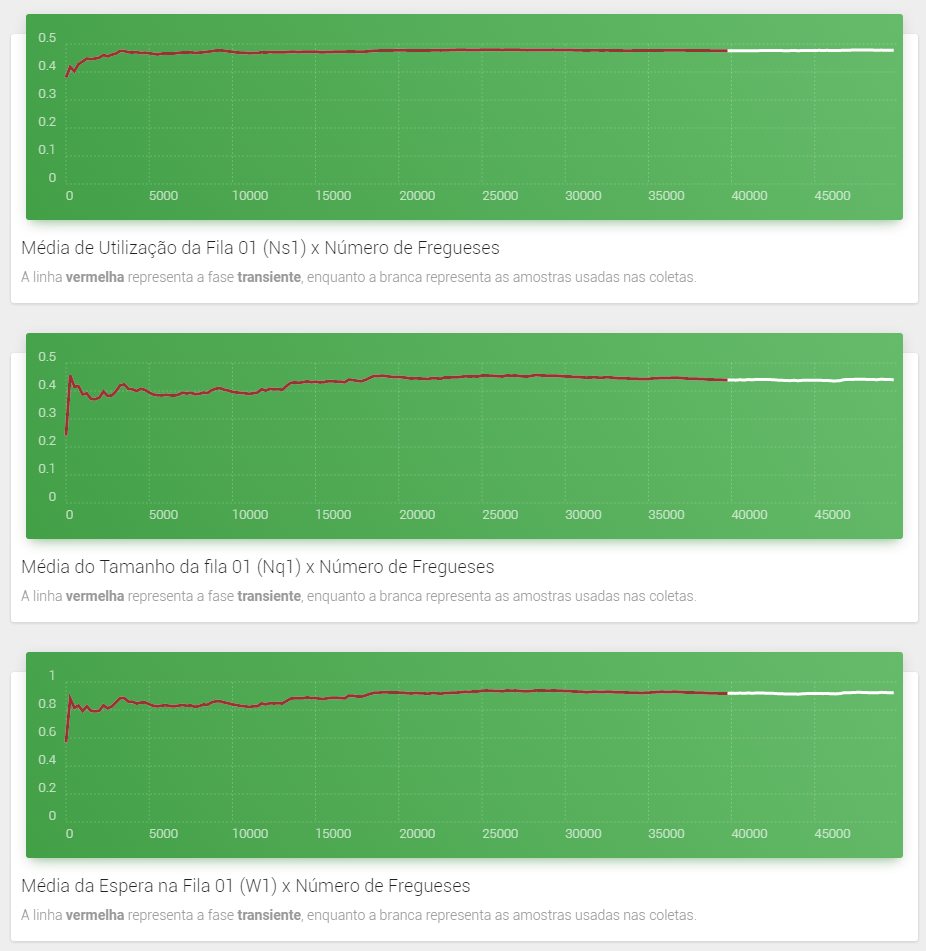
\includegraphics[width=1\textwidth]{./graficos/transient/mediasfilas1rho095.png}
\vspace{-10mm}
\caption{Métricas da Fila 1 com $\rho=0.95$ estabilizam mais rapidamente.}
\end{figure}

\begin{figure}[H]
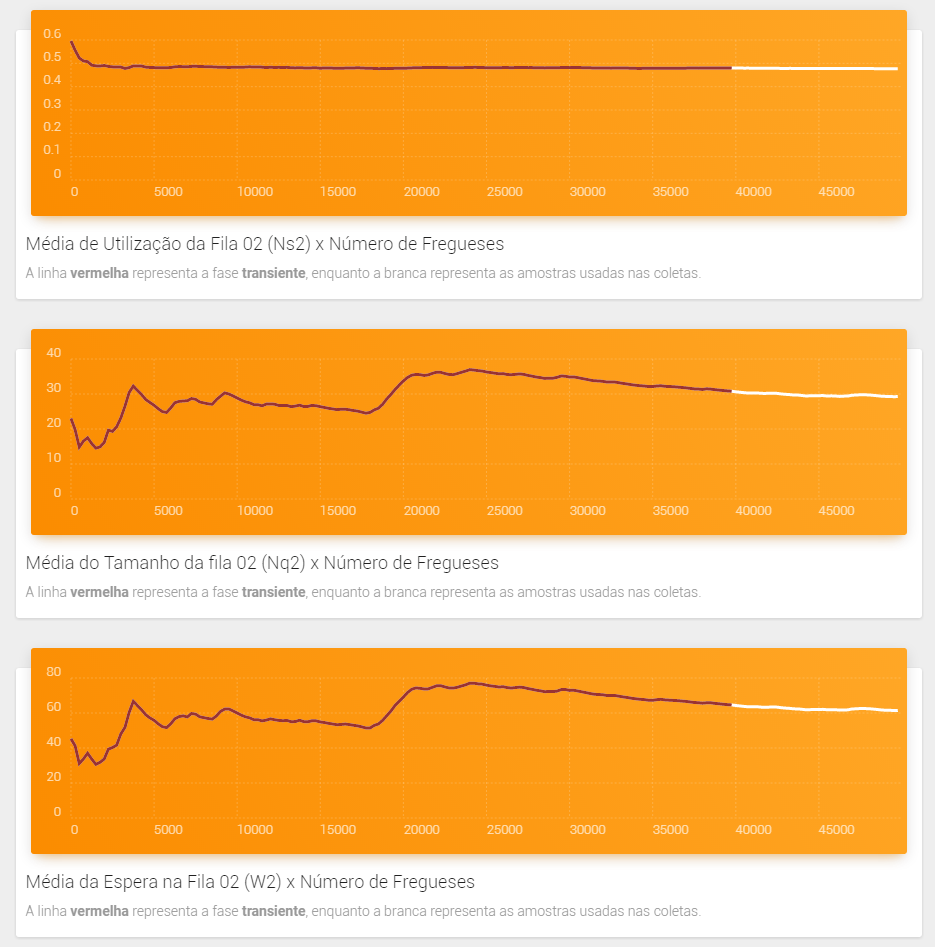
\includegraphics[width=1\textwidth]{./graficos/transient/mediasfilas2rho095.png}
\vspace{-10mm}
\caption{Métricas da Fila 2 com $\rho=0.95$ demoram mais pra estabilizar.}
\end{figure}

Para determinar o tamanho da \textbf{fase transiente} de modo que
todo o sistema já estivesse em equilíbrio foi necessário que ela fosse pelo menos do tamanho da fase instável da medida mais crítica. De acordo com os testes, foram as métricas da  \textbf{Fila 2}: $\overline{N_{q2}}$, $\overline{W2}$ e V[W2].

Tendo os parâmetros mais críticos definidos, foram executados diversos testes para se determinar o tamanho da fase transiente. Apesar da semente não ser tão relevante no método \emph{batch}, foram executados mais de 100 testes com diferentes sementes e anotados os momentos perceptíveis de equilíbrio das mesmas, assim como o maior valor de equilíbrio encontrado.

As seguintes imagens mostram como a fase transiente varia dependendo da semente utilizada:

\begin{figure}[H]
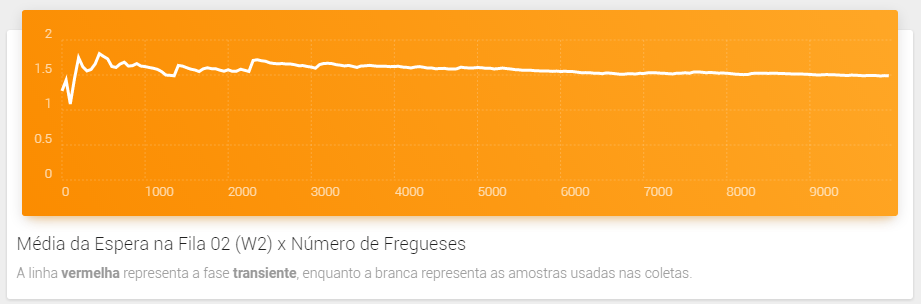
\includegraphics[width=1\textwidth]{./graficos/transient/transientSeed1.png}
\vspace{-10mm}
\caption{Execução com 10 mil fregueses, $\rho=0.4$ e seed = ``1''.}
\end{figure}

\begin{figure}[H]
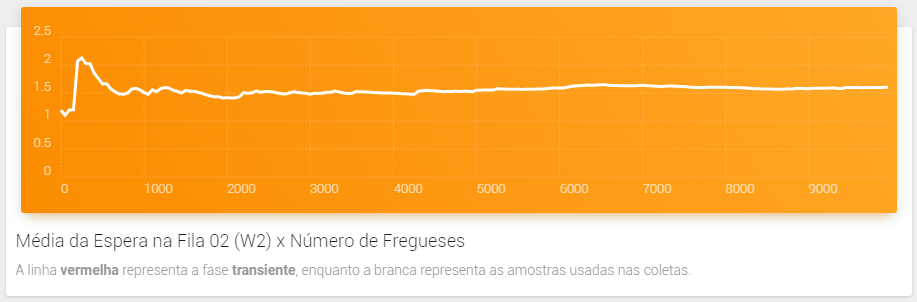
\includegraphics[width=1\textwidth]{./graficos/transient/transientSeed2.png}
\vspace{-10mm}
\caption{Execução com 10 mil fregueses, $\rho=0.4$ e seed = ``2''.}
\end{figure}

\begin{figure}[H]
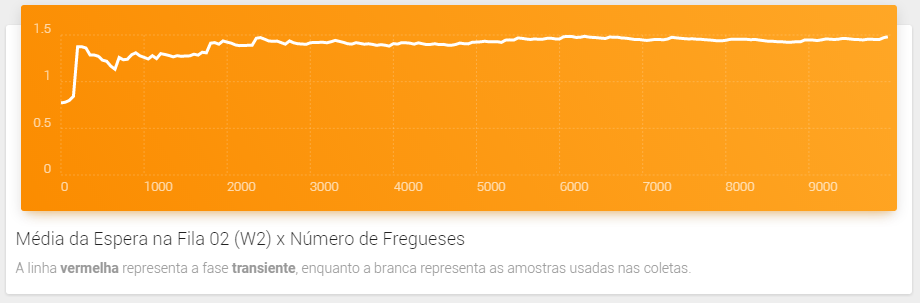
\includegraphics[width=1\textwidth]{./graficos/transient/transientSeed4.png}
\vspace{-10mm}
\caption{Simulação com 10 mil fregueses, $\rho=0.4$ e seed = ``4''.}
\end{figure}

\begin{figure}[H]
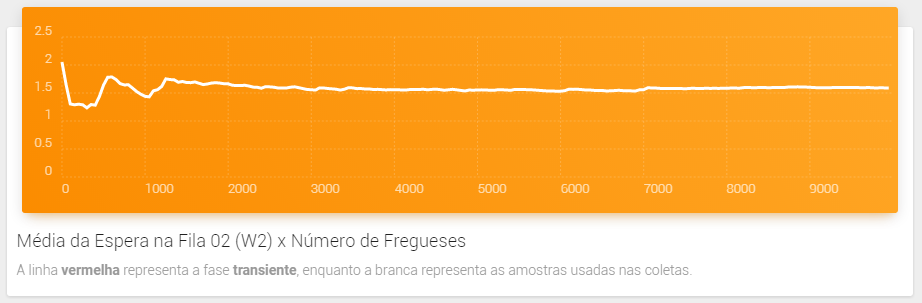
\includegraphics[width=1\textwidth]{./graficos/transient/transientSeed5.png}
\vspace{-10mm}
\caption{Execução com 10 mil fregueses, $\rho=0.4$ e seed = ``5''.}
\end{figure}
 
É possível observar nos gráficos acima que, apesar do sistema estabilizar em momentos semelhantes, ainda existe uma diferença dependendo da semente. Através destes testes foi possível garantir que o tamanho da fase transiente é independente da semente escolhida, pois cada um retornou um resultado completamente independente do anterior. O pior caso de todos os testes definiu qual seria a fase transiente.

Finalmente, foram escolhidos tamanhos para a fase transiente de diferentes intervalos de $\rho$, sempre observando mais atentamente o $\overline{\textbf{W2}}$ e $\textbf{V[W2]}$, conforme mostra a tabela a seguir.

\begin{center}
\begin{tabular}[H]{ c c }
  \hline
  Intervalo de $\rho$ & Tamanho da fase transiente \\
  \hline
  $0   < \rho \leq 0.4 $  & 10000 \\
  $0.4 < \rho \leq 0.6 $  & 15000 \\
  $0.6 < \rho \leq 0.8 $  & 20000 \\
  $0.8 < \rho < 1 $  & 40000 \\
  \hline
\end{tabular}
\end{center}

Como quanto maior o $\rho$, mais demorado é o momento de estabilização das filas. O tamanho da fase transiente da tabela acima reflete esta característica. É importante ressaltar que caso o $\rho$ esteja muito próximo de 1, com valores como 0,999, a fila demoraria muito mais de que 40 mil fregueses para estabilizar, ou até mesmo nem estabilizaria em um tempo viável. Por isto, estes casos não foram considerados na simulação.

Pelo fato das fases transientes escolhidas terem um tamanho relativamente significativo, foi percebido que seria muito ineficiente utilizar o método replicativo, pois desta forma o \textbf{Total de Fregueses} seria aumentado significativamente a cada rodada adicionada à simulação. Este foi o maior motivo para que o método \emph{batch} fosse escolhido para a execução do simulador.

\section{Influência da Fase Transiente na Qualidade das Medidas}

Comprovando os testes feitos anteriormente para escolher as fases transientes para cada um dos valores possíveis de $\rho$ ($\rho_1 + \rho_2$), é possível ver pelos testes abaixo como o uso de fase transiente proporcionou resultados melhores, principalmente em casos onde o número de fregueses no geral é baixo.

\begin{center}

\begin{table}[H]
\caption{Simulação com 100 fregueses, 10 rodadas, $\rho=0,6$ e seed ``test''.}
\bigskip
\begin{tabular}{ c c c c c c c }
  \hline
  \textbf{Resultado} & $N_{q1}$ & $W_1$ & $N_{q2}$ & $N_2$ & $W_2$ & $T_2$ \\
  \hline
  Analítico & 0,1286 & 0,4286 & 1,0929 & 1,3929 & 3,6429 & 4,6429 \\
  Transiente & \textbf{0,1190} & 0,4002 & \textbf{1,0040} & \textbf{1,3120} & \textbf{3,5256} & \textbf{4,5818}\\
  Sem Transiente & 0,1130 & \textbf{0,4140} & 0,9250 & 1,2120 & 3,0925 & 4,0740 \\
  \hline
\end{tabular}
\end{table}

\begin{table}[H]
\caption{Simulação com 100 fregueses, 10 rodadas, $\rho$ = 0,8 e seed ``test''.}
\bigskip
\begin{tabular}{ c c c c c c c }
  \hline
  \textbf{Resultado} & $N_{q1}$ & $W_1$ & $N_{q2}$ & $N_2$ & $W_2$ & $T_2$ \\
  \hline
  Analítico & 0,2667 & 0,6667 & 4,2667 & 4,6667 & 10,6667 & 11,6667 \\
  Transiente & \textbf{0,2480} & \textbf{0,6328} & \textbf{3,1870} & \textbf{3,5670} & \textbf{8,1668} & \textbf{9,1445}\\
  Sem Transiente & 0,2420 & 0,6154 & 2,9470 & 3,3510 & 7,5082 & 8,4897 \\
  \hline
\end{tabular}
\end{table}
\end{center}
\vspace{-3em}

Como podemos ver nestes dois exemplos, a simulação com o uso do período transiente obteve resultados mais próximos das métricas analíticas. Entretanto, estas diferenças só são observadas em maioria nos casos onde temos simulações com um número pequeno de fregueses no geral. Isso se deve ao fato de que, quanto maior o número de fregueses que existem no caso rodado, maior será o número de fregueses ``estabilizados'', com métricas que oscilam menos do que os fregueses do período transiente. Por conta disso, na hora de calcular a média, a quantidade elevada deles comparada com o número de fregueses transientes acaba diminuindo o efeito destes últimos fregueses na esperança de cada uma das métricas, convergindo mais rapidamente para os resultados esperados.

\section{Funcionamento}

Para implementar a fase transiente na simulação, foi necessário identificar, de alguma maneira, se o consumidor que estiver entrando no sistema neste instante é um dos primeiros fregueses do sistema, respeitando o tamanho da fase transiente previamente definido. Para isso, foi utilizado o campo identificador do objeto \emph{Customer}. Como podemos ver abaixo, a variável que controla o número a ser utilizado como identificado para o próximo freguês que chegar no sistema não começa em 0, e sim em $-nTransient$, que é igual ao tamanho da fase transiente. Vale lembrar que em \emph{JavaScript} é possível endereçar \emph{arrays} com índices negativos.

\begin{lstlisting}
  // Indice -1 representa um "round" reservado para a fase transiente
  Nq1Avg[-1] = 0;
  Ns1Avg[-1] = 0;
  N1Avg[-1] = 0;
  Nq2Avg[-1] = 0;
  Ns2Avg[-1] = 0;
  N2Avg[-1] = 0;
  W1Avg[-1] = 0;
  X1Avg[-1] = 0;
  T1Avg[-1] = 0;
  W2Avg[-1] = 0;
  X2Avg[-1] = 0;
  T2Avg[-1] = 0;

  let nextCustomerId = -nTransient; // Variavel que representa o proximo ID que deve ser usado na criacao  de um fregues. IDs menores que 0 representam o periodo transiente
\end{lstlisting}

Por conta desta utilização de identificadores negativos, é fácil saber se um freguês é transiente ou não, bastando verificar se este parâmetro é menor que zero. Quando a simulação calcula cada uma das métricas de um freguês que faz parte do período transiente, seus valores são salvos na ``rodada'' -1, para serem posteriormente exibidos no gráfico como a fase transiente (representada em vermelho). No entanto, vale lembrar que os mesmos são armazenados apenas para serem exibidos como uma informação interessante nos gráficos e não são utilizados nos cálculos das métricas (Médias e Variâncias).

%%%%%%%%%%%%%
% Análise
%%%%%%%%%%%%%
%tabelas com resultados e comentários pertinentes
\chapter{Resultados}

Nesta seção serão comentados os resultados obtidos e comparados com os valores analíticos. Serão também indicados os valores dos parâmetros utilizados para cada $\rho$ ($\rho_1 + \rho_2$), para satisfazer aos requisitos mínimos. Por último, serão discutidas algumas observações interessantes e peculiaridades da simulação.

\section{Tabela de Valores Analíticos}

Os resultados analíticos para diversos valores de $\rho$ são mostrados na tabela a seguir. Estes valores foram calculados analiticamente através de fórmulas conhecidas, e servirão como forma de comparação com os resultados obtidos pelo simulador. O $\rho$ na tabela se refere a utilização geral do sistema, ou seja, $\rho_1 + \rho_2$.

\begin{center}
\begin{tabular}{ c c c c c c c }
    \hline
	\textbf{$\rho$} & \textbf{E[W1]} & \textbf{E[Nq1]} & \textbf{E[T2]} & \textbf{E[N2]} & \textbf{E[W2]} & \textbf{E[Nq2]} \\
	\hline
	0,9 & 0,81818 & 0,36818 & 26,36364 & 11,86364 & 25,36364 & 11,41364 \\
	0,8 & 0,66667 & 0,26667 & 11,66667 & 4,66667 & 10,66667 & 4,26667 \\
	0,6 & 0,42857 & 0,12857 & 4,64286 & 1,39286 & 3,64286 & 1,09286 \\
	0,4 & 0,25000 & 0,05000 & 2,50000 & 0,50000 & 1,50000 & 0,30000 \\
	0,2 & 0,11111 & 0,01111 & 1,52778 & 0,15278 & 0,52778 & 0,05278 \\
	\hline
\end{tabular}
\end{center}

\section{Simulação com Diferentes Valores de $\rho$}

Para todos os valores de $\rho$ que testamos, conseguimos intervalos de confiança de 95\% que incluíam os valores analíticos, com precisão melhor do que 5\%. O valor dos parâmetros utilizado para cada teste será detalhado a seguir.

\subsection{Para $\rho$ = 0,2}
Para $\rho$ = 0,2, utilizamos com os seguintes parâmetros:

\vspace{-5mm}
\begin{center}
\begin{tabular}{ c c }
  \hline
  \textbf{Parâmetro} & \textbf{Valor}\\
  \hline
  Utilização ($\rho$) & 0,2\\
  Fase transiente & 10.000\\
  Nº de rodadas & 3.100\\
  Nº de fregueses & 100\\
  \hline
\end{tabular}
\end{center}

Os resultados obtidos no simulador foram:
\begin{figure}[H]
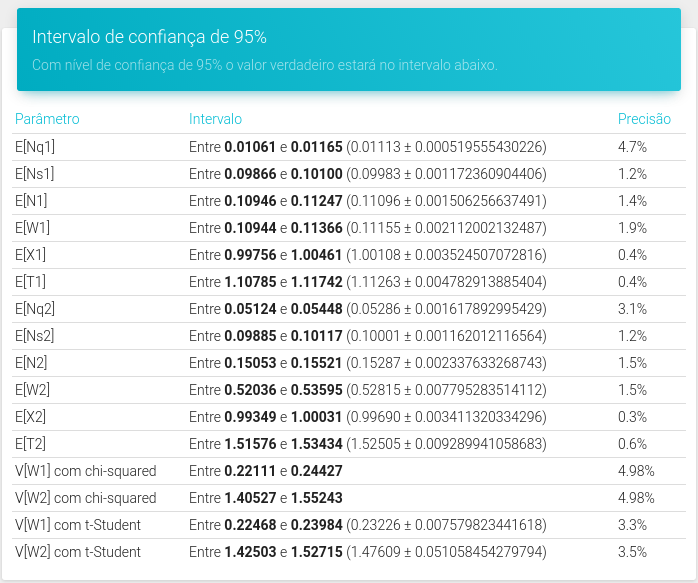
\includegraphics[width=1\textwidth]{./graficos/cap4/rho02.png}
\vspace{-10mm}
%\caption{Simulação com $\rho$ = 1.3 e 100 mil fregueses.}
\end{figure}

Comparando com os resultados analíticos, observamos que os valores analíticos estão de fato dentro do intervalo de confiança obtido:

\vspace{-5mm}
\begin{center}
\begin{tabular}{ c c c }
  \hline
  \textbf{Métrica} & \textbf{Valor Analítico} & \textbf{Intervalo de Confiança} \\
  \hline
  $N_{q1}$ & 0,01111 & Entre 0,01061 e 0,01165 \\
  $W_1$    & 0,11111 & Entre 0,10944 e 0,11366 \\
  $N_{q2}$ & 0,05278 & Entre 0,05124 e 0,05448 \\
  $N_2$    & 0,15278 & Entre 0,15053 e 0,15521 \\
  $W_2$    & 0,52778 & Entre 0,52036 e 0,53595 \\
  $T_2$    & 1,52778 & Entre 1,51576 e 1,53434 \\
  \hline
\end{tabular}
\end{center}

\subsection{Para $\rho$ = 0,4}
Para $\rho$ = 0,4, foram utilizados os seguintes parâmetros:

\vspace{-5mm}

\begin{center}
\begin{tabular}{ c c }
  \hline
  \textbf{Parâmetro} & \textbf{Valor}\\
  \hline
  Utilização ($\rho$) & 0,4\\
  Fase transiente & 10.000\\
  Nº de rodadas & 3.100\\
  Nº de fregueses & 100\\
  \hline
\end{tabular}
\end{center}

Os resultados obtidos no simulador foram:
\begin{figure}[H]
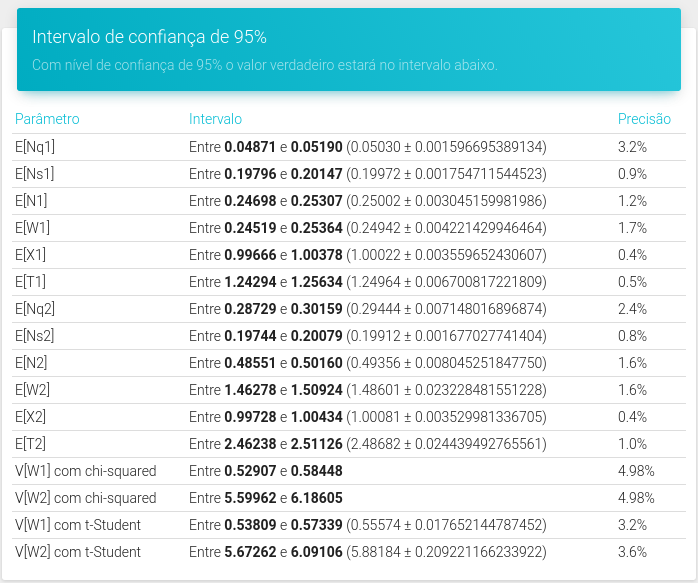
\includegraphics[width=1\textwidth]{./graficos/cap4/rho04.png}
\vspace{-10mm}
%\caption{Simulação com $\rho$ = 1.3 e 100 mil fregueses.}
\end{figure}

Comparando com os resultados analíticos, observamos que os valores analíticos estão de fato dentro do intervalo de confiança obtido:

\vspace{-5mm}
\begin{center}
\begin{tabular}{ c c c }
  \hline
  \textbf{Métrica} & \textbf{Valor Analítico} & \textbf{Intervalo de Confiança} \\
  \hline
  $N_{q1}$ & 0,05000 & Entre 0,04871 e 0,05190 \\
  $W_1$    & 0,25000 & Entre 0,24519 e 0,25364 \\
  $N_{q2}$ & 0,30000 & Entre 0,28729 e 0,30159 \\
  $N_2$    & 0,50000 & Entre 0,48551 e 0,50160 \\
  $W_2$    & 1,50000 & Entre 1,46278 e 1,50924 \\
  $T_2$    & 2,50000 & Entre 2,46238 e 2,51126 \\
  \hline
\end{tabular}
\end{center}

\subsection{Para $\rho$ = 0,6}
Para $\rho$ = 0,6, foram utilizados os seguintes parâmetros:

\vspace{-5mm}
\begin{center}
\begin{tabular}{ c c }
  \hline
  \textbf{Parâmetro} & \textbf{Valor}\\
  \hline
  Utilização ($\rho$) & 0,6\\
  Fase transiente & 15.000\\
  Nº de rodadas & 3.100\\
  Nº de fregueses & 150\\
  \hline
\end{tabular}
\end{center}

Os resultados obtidos no simulador foram:
\begin{figure}[H]
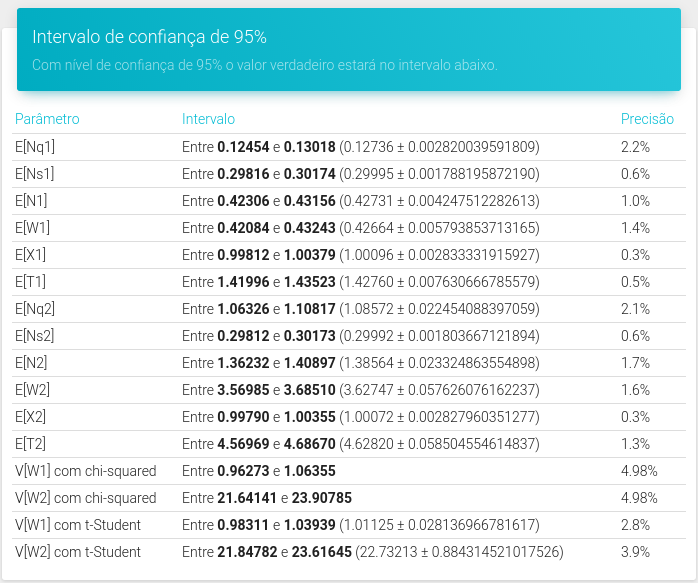
\includegraphics[width=1\textwidth]{./graficos/cap4/rho06.png}
\vspace{-10mm}
%\caption{Simulação com $\rho$ = 1.3 e 100 mil fregueses.}
\end{figure}

Comparando com os resultados analíticos, observamos que os valores analíticos estão de fato dentro do intervalo de confiança obtido:

\vspace{-5mm}
\begin{center}
\begin{tabular}{ c c c }
  \hline
  \textbf{Métrica} & \textbf{Valor Analítico} & \textbf{Intervalo de Confiança} \\
  \hline
  $N_{q1}$ & 0,12857 & Entre 0,12454 e 0,13018 \\
  $W_1$    & 0,42857 & Entre 0,42084 e 0,43243 \\
  $N_{q2}$ & 1,09286 & Entre 1,06326 e 1,10817 \\
  $N_2$    & 1,39286 & Entre 1,36232 e 1,40897 \\
  $W_2$    & 3,64286 & Entre 3,56985 e 3,68510 \\
  $T_2$    & 4,64286 & Entre 4,56969 e 4,68670 \\
  \hline
\end{tabular}
\end{center}

\subsection{Para $\rho$ = 0,8}
Para $\rho$ = 0,8, foram utilizados os seguintes parâmetros:

\vspace{-5mm}
\begin{center}
\begin{tabular}{ c c }
  \hline
  \textbf{Parâmetro} & \textbf{Valor}\\
  \hline
  Utilização ($\rho$) & 0,8\\
  Fase transiente & 20.000\\
  Nº de rodadas & 3.100\\
  Nº de fregueses & 180\\
  \hline
\end{tabular}
\end{center}

Os resultados obtidos no simulador foram:
\begin{figure}[H]
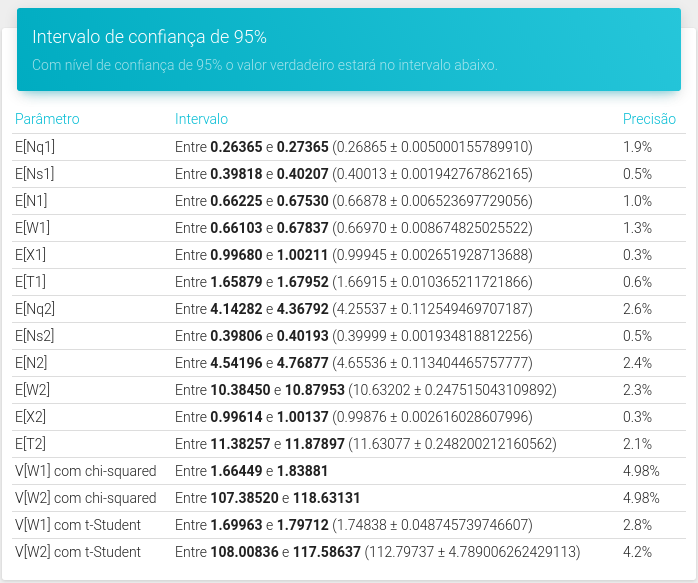
\includegraphics[width=1\textwidth]{./graficos/cap4/rho08.png}
\vspace{-10mm}
%\caption{Simulação com $\rho$ = 1.3 e 100 mil fregueses.}
\end{figure}

Comparando com os resultados analíticos, observamos que os valores analíticos estão de fato dentro do intervalo de confiança obtido:

\vspace{-5mm}
\begin{center}
\begin{tabular}{ c c c }
  \hline
  \textbf{Métrica} & \textbf{Valor Analítico} & \textbf{Intervalo de Confiança} \\
  \hline
  $N_{q1}$ & 0,26667 & Entre 0,26365 e 0,27365 \\
  $W_1$    & 0,66667 & Entre 0,66103 e 0,67837 \\
  $N_{q2}$ & 4,26667 & Entre 4,14282 e 4,36792 \\
  $N_2$    & 4,66667 & Entre 4,54196 e 4,76877 \\
  $W_2$    & 10,66667 & Entre 10,38450 e 10,87953 \\
  $T_2$    & 11,66667 & Entre 11,38257 e 11,87897 \\
  \hline
\end{tabular}
\end{center}



\subsection{Para $\rho$ = 0,9}
Para $\rho$ = 0,9, foram utilizados os seguintes parâmetros:

\vspace{-5mm}
\begin{center}
\begin{tabular}{ c c }
  \hline
  \textbf{Parâmetro} & \textbf{Valor}\\
  \hline
  Utilização ($\rho$) & 0,9\\
  Fase transiente & 40.000\\
  Nº de rodadas & 3.100\\
  Nº de fregueses & 200\\
  \hline
\end{tabular}
\end{center}

Os resultados obtidos no simulador foram:

\begin{figure}[H]
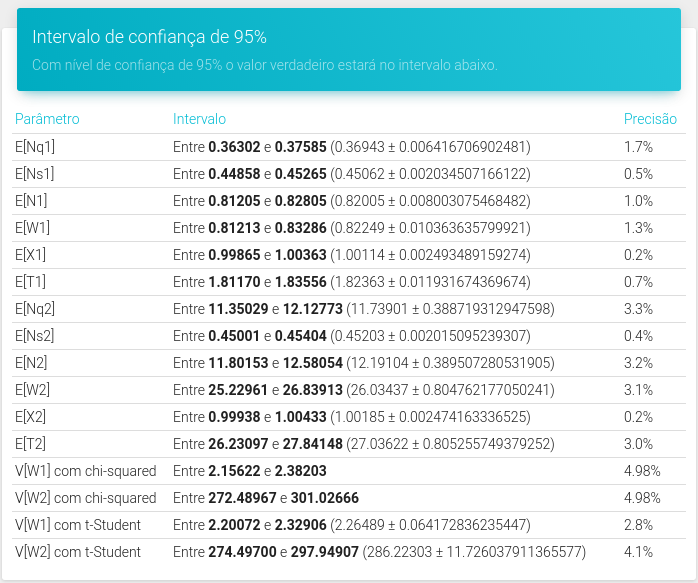
\includegraphics[width=1\textwidth]{./graficos/cap4/rho09.png}
\vspace{-10mm}
%\caption{Simulação com $\rho$ = 1.3 e 100 mil fregueses.}
\end{figure}

Comparando com os resultados analíticos, observamos que os valores analíticos estão de fato dentro do intervalo de confiança obtido:

\vspace{-5mm}
\begin{center}
\begin{tabular}{ c c c }
  \hline
  \textbf{Métrica} & \textbf{Valor Analítico} & \textbf{Intervalo de Confiança} \\
  \hline
  $N_{q1}$ & 0,36818 & Entre 0,36302 e 0,37585 \\
  $W_1$    & 0,81818 & Entre 0,81213 e 0,83286 \\
  $N_{q2}$ & 11,41364 & Entre 11,35029 e 12,12773 \\
  $N_2$    & 11,86364 & Entre 11,80153 e 12,58054 \\
  $W_2$    & 25,36364 & Entre 25,22961 e 26,83913 \\
  $T_2$    & 26,36364 & Entre 26,23097 e 27,84148 \\
  \hline
\end{tabular}
\end{center}

\section{Observações sobre Parâmetros}

Ao realizar mudanças em alguns dos parâmetros, pudemos observar individualmente o efeito deles nos resultados da simulação. Segue abaixo análises sobre alguns desses parâmetros, e como os resultados observados são úteis para entender mais profundamente o funcionamento do sistema simulado.

\subsection{Efeitos da Variação do Número de Rodadas}

Mantendo o mesmo número total de fregueses, mas diminuindo o número de rodadas e aumentando o número de fregueses por rodada, o intervalo de confiança parece variar mais. Com um número alto de rodadas, o intervalo de confiança se mantém mais estável, variando menos ao rodar o simulador diversas vezes.

Fizemos testes com um total de 200.000 fregueses, com diferentes números de rodadas. Para cada número de rodadas, rodamos o simulador diversas vezes, e observamos o intervalo no qual a precisão do intervalo de confiança variava. Executamos 100 testes para cada caso, e, para V[W2], o parâmetro que mais variava, pegamos o valor mínimo e máximo da precisão. A taxa de utilização geral utilizada foi de 0,4 para todos os testes. Os resultados podem ser vistos na tabela e gráfico abaixo.


\begin{table}[H]
\begin{center}
\begin{tabular}{ c c c }
  \hline
  \textbf{Rodadas} & \textbf{Freg. por rodada} & \textbf{Variação da precisão} \\
  \hline
  10  & 20000 & De 3.0\% a 10.6\% \\
  20  & 10000 & De 3.3\% a 8.9\% \\
  40  & 5000  & De 3.7\% a 7.0\% \\
  80  & 2500  & De 4.0\% a 6.7\% \\
  160 & 1250  & De 4.0\% a 7.2\% \\
  320 & 625   & De 4.3\% a 6.8\% \\
  640 & 312   & De 4.5\% a 6.7\% \\
  1280 & 156  & De 4.2\% a 6.1\% \\
  2560 & 78   & De 4.2\% a 5.6\% \\
  \hline
\end{tabular}
\caption{Variação da precisão do IC de V[$W_2$]}
\end{center}
\end{table}


\begin{figure}[H]
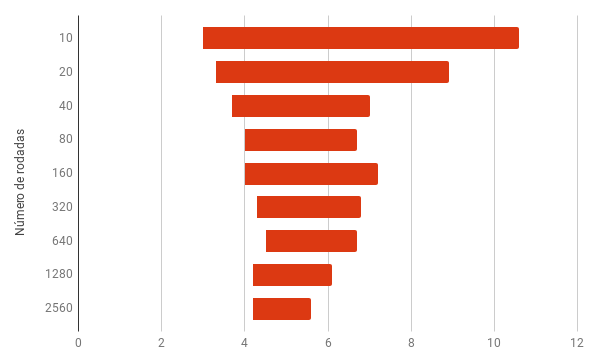
\includegraphics[width=1\textwidth]{./graficos/variacao_ic_w2.png}
\vspace{-10mm}
\caption{Variação da precisão do IC de V[$W_2$]}
\end{figure}


Uma razão para isso seria que, com mais rodadas, teremos mais amostras para o cálculo do intervalo de confiança. Com isso, o desvio padrão, fator multiplicativo usado no cálculo dos extremos do intervalo de confiança, será menor, fazendo com que o intervalo seja sempre menor, implicando numa precisão melhor.


\subsection{Valores Muito Altos de $\rho$}

Para valores muito altos de $\rho$, pudemos notar, pelos gráficos, que a fila demora muito mais para convergir para o valor analítico. Mostramos abaixo alguns testes. A fase transiente foi definida como 0 para estes testes.

\vspace{10mm}

\begin{figure}[H]
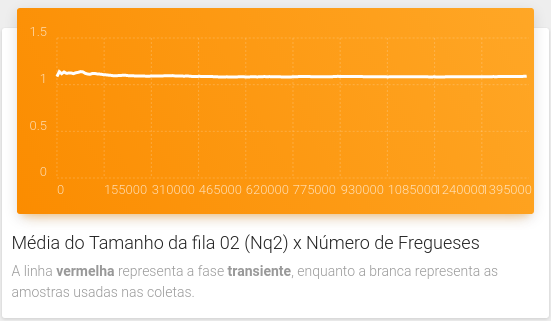
\includegraphics[width=1\textwidth]{./graficos/rho06compara.png}
\vspace{-10mm}
\caption{Média de $N_{q2}$ por freguês com $\rho$ = 0,6}
\end{figure}

\begin{figure}[H]
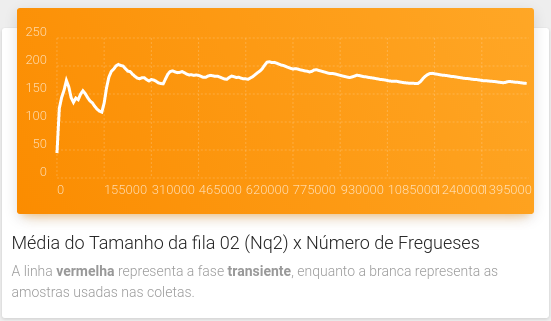
\includegraphics[width=1\textwidth]{./graficos/rho099compara.png}
\vspace{-10mm}
\caption{Média de $N_{q2}$ por freguês com $\rho$ = 0,99}
\end{figure}

Podemos ver que, para 400.000 fregueses, o teste com taxa de utilização do sistema 0,6, $N_{q2}$ se manteve muito mais estável, enquanto que no teste com taxa 0,99, $N_{q2}$ pareceu começar a convergir, mas ainda não se estabilizou por completo, em todo este intervalo.


%%%%%%%%%%%%%
% Otimização
%%%%%%%%%%%%%
\chapter{Otimização}

Para encontrar os parâmetros ótimos da simulação que cumpram todos os requisitos, foram necessárias algumas técnicas e a automatização de alguns testes, além de testes manuais. Os parâmetros que poderiam ser alterados para otimizar o \textbf{fator mínimo} são: a \textbf{fase transiente}, o \textbf{número de rodadas}, \textbf{número de fregueses por rodada}.

\section{Apresentação do Método}

Uma rotina automatizada foi escrita para receber um valor N como entrada e rodar a simulação com K rodadas e M fregueses um número N de vezes, com sementes diferentes. Depois disso, a rotina exibe quantos testes estavam fora do critério limite de 5\% para a precisão das métricas, além das médias estarem dentro do intervalo de confiança de 95\%. Entretanto, para testar valores de parâmetros de entrada, testes manuais eram feitos, por serem produzidos em quantidade reduzida, apenas para testar se os parâmetros em questão eram candidatos plausíveis para um teste mais extenso, por meio da rotina automatizada.

\begin{lstlisting}[caption={Rotina automatizada de teste.},captionpos=b]
    let nPrecisionOK = 0;
    let nTests = 1000;
    
    let startTime = new Date().getTime();
    for (let i=0; i<nTests; i++){
    	if(this.runRounds(nTransient, nCustomers, nRounds, lambda, mi))
    		nPrecisionOK++;
    }
    let endTime = new Date().getTime();
    
    $.notifyClose();
    document.getElementById("simTitle").innerHTML = 
        "Simulacao com "+((endTime -  startTime)/1000)+" segundos<br>" + nPrecisionOK + "/" + nTests + " casos com precisao <= 5%";
\end{lstlisting}

Definimos o seguinte critério para considerar os parâmetros válidos e utilizar como possíveis candidatos para o Fator Mínimo: se, nesses testes, 95\% das execuções cumpriram os critérios (este critério foi arbitrário, poderia ser 90\% ou mesmo 100\% por exemplo), então consideramos os parâmetros válidos. No entanto, cada vez que o número de testes falhos excede o máximo de 5\% que definimos, alguns dos parâmetros de entrada da simulação eram alterados, a fim de achar um equilíbrio entre o número de fregueses totais da simulação e poucos casos acima de 5\% de precisão, respeitando o mínimo de 95\%.

\subsection{Fase Transiente}

A \textbf{fase transiente} já foi otimizada ao limite conforme explicado e demonstrado na seção 3. Apesar disso, foram realizados testes para tentar reduzir ainda mais a fase transiente. No entanto, não foi possível reduzir mais. Os testes ao longo deste capítulo mostram que os valores utilizados para fase transiente são os mesmos que os definidos na seção 3.

\subsection{Número de Rodadas}

Observamos que a precisão dos intervalos de confiança de V[W1] e V[W2] com \emph{chi-squared} é função apenas do número de rodadas, e não dos outros parâmetros. Por isso, determinamos o valor mínimo do número de rodadas para que essas duas precisões ficassem abaixo de 5\%.
Com 3071 rodadas, a precisão da chi-squared é 4.99921\%. Dessa forma, este número foi um limitante inferior para nosso número de rodadas em todos os testes.


\subsection{Número de Fregueses}

Por conta da limitação do valor mínimo do número de rodadas, o \textbf{número de fregueses} foi o parâmetro mais alterado nos testes de otimização. Como existe um mínimo para que a distribuição de fregueses por rodada se aproxime de uma normal, o mínimo de fregueses por rodada também teve um limite na sua redução para que a simulação cumprisse os critérios mínimos.

\section{Fatores Mínimos}

Após as otimizações realizadas, os fatores mínimos seguintes foram encontrados para cada $\rho$ ($\rho_1 + \rho_2$). A cada execução, as sementes foram diferentes.

% RHO 0.2
\subsection{Fator Mínimo para $\rho$ = 0,2}
\begin{center}
\begin{tabular}{ c c }
  \hline
  \textbf{Parâmetro} & \textbf{Valor}\\
  \hline
  Utilização ($\rho$) & 0,2\\
  Fase transiente & 10.000\\
  Nº de rodadas & 3.080\\
  Nº de fregueses & 100\\
  \hline
  \textbf{Fator mínimo} & 318.000\\
  \hline
\end{tabular}
\end{center}

Em 100 testes manuais, apenas o $N_{q1}$ teve dois testes com precisão 5,1\% e 5,2\%, respectivamente. Em 1000 testes automatizados, tivemos 951 casos que ficaram com todas as métricas com precisão menor ou igual 5\%, representando 95,1\% de casos dentro das restrições.


% RHO 0.4
\subsection{Fator Mínimo para $\rho$ = 0,4}
\begin{center}
\begin{tabular}{ c c }
  \hline
  \textbf{Parâmetro} & \textbf{Valor}\\
  \hline
  Utilização ($\rho$) & 0,4\\
  Fase transiente & 10.000\\
  Nº de rodadas & 3.071\\
  Nº de fregueses & 65\\
  \hline
  \textbf{Fator mínimo} & 209.615\\
  \hline
\end{tabular}
\end{center}

Em 100 testes manuais, apenas a V[W2] ficou fora do limite de precisão, 4 vezes, mas com valores entre 5,01\% e 5,3\%. Em 1000 testes automatizados, tivemos 955 casos que ficaram com todas as métricas com precisão menor ou igual 5\%, representando 95,5\% de casos dentro das restrições.


% RHO 0.6
\subsection{Fator Mínimo para $\rho$ = 0,6}
\begin{center}
\begin{tabular}{ c c }
  \hline
  \textbf{Parâmetro} & \textbf{Valor}\\
  \hline
  Utilização ($\rho$) & 0,6\\
  Fase transiente & 15.000\\
  Nº de rodadas & 3.071\\
  Nº de fregueses & 110\\
  \hline
  \textbf{Fator mínimo} & 352.810\\
  \hline
\end{tabular}
\end{center}

Em 1000 testes automatizados, tivemos 959 casos que ficaram com todas as métricas com precisão menor ou igual 5\%, representando 95,9\% de casos dentro das restrições.

% RHO 0.8
\subsection{Fator Mínimo para $\rho$ = 0,8}
\begin{center}
\begin{tabular}{ c c }
  \hline
  \textbf{Parâmetro} & \textbf{Valor}\\
  \hline
  Utilização ($\rho$) & 0,8\\
  Fase transiente & 20.000\\
  Nº de rodadas & 3.071\\
  Nº de fregueses & 55\\
  \hline
  \textbf{Fator mínimo} & 188.905\\
  \hline
\end{tabular}
\end{center}

Em 1000 testes automatizados, tivemos 975 casos que ficaram com todas as métricas com precisão menor ou igual 5\%, representando 97,5\% de casos dentro das restrições.

% RHO 0.9
\subsection{Fator Mínimo para $\rho$ = 0,9}
\begin{center}
\begin{tabular}{ c c }
  \hline
  \textbf{Parâmetro} & \textbf{Valor}\\
  \hline
  Utilização ($\rho$) & 0,9\\
  Fase transiente & 40.000\\
  Nº de rodadas & 3.071\\
  Nº de fregueses & 55\\
  \hline
  \textbf{Fator mínimo} & 208.905\\
  \hline
\end{tabular}
\end{center}

Em 1000 testes automatizados, tivemos 984 casos que ficaram com todas as métricas com precisão menor ou igual 5\%, representando 98,4\% de casos dentro das restrições.

% CONCLUSOES
\section{Comentários Finais}

Os testes manuais se resumiram a testar alguns candidatos a \textbf{fator} mínimo, antes de ser feita uma análise em maior escala. Após a escolha, pudemos fazer uso dos testes automatizados, onde cada uma das taxas de utilização pôde ser testada de maneira mais extensa. Com a execução dos testes automatizados, a porcentagem de resultados que respeitaram as restrições impostas nos testes foi alta. A ordem de grandeza do fator mínimo foi a mesma para todos os valores de $\rho$, com os valores oscilando entre valores que foram considerados aceitáveis, em torno de 190 mil a 350 mil fregueses. Por conta destes fatores, foi considerado que o nível de otimização do simulador é satisfatório para o sistema de filas proposto.

%%%%%%%%%%%%%
% Conclusão
%%%%%%%%%%%%%
\chapter{Conclusão}

Construir todo este projeto, desde sua concepção até sua finalização, foi essencial para consolidar a matéria vista em aula, e para compreender na prática todas as dificuldades e objetivos por trás de elaborar uma simulação. O aprendizado, resultado, corretude e visualização da simulação foram bastante sido satisfatórios para o grupo; porém, diversas dificuldades foram encontradas durante a realização do projeto.


\section{Dificuldades na Implementação e Otimização}

Inicialmente, a implementação da simulação estava complexa. O primeiro protótipo do sistema era muito ineficiente e usava bastante memória, por conta da implementação de uma lista de eventos grande, sem remoção, e com 6 tipos de eventos. Dessa forma, era impossível o simulador processar mais de 100 mil fregueses em tempo hábil. 

Após tirar dúvidas com o professor e refazer o funcionamento da simulação do zero sem criar uma lista grande de eventos e calculando as médias incrementalmente, foi possível executar a simulação com uma quantidade bem grande de fregueses e rodadas, com tempo e memória aceitáveis, sendo possível rodar até 5 milhões de fregueses em menos de 2 minutos.

Finalmente, após uma terceira otimização das estruturas utilizadas e da complexidade de alguns cálculos, foi possível alcançar o limite de 70 milhões de fregueses em menos de 4 minutos, além de uma complexidade de tempo linear em relação ao número total de fregueses, conforme foi dito na primeira seção.

Outro desafio foi estruturar de maneira compreensível e simples todo o código da simulação e geração de métricas. Isto acarretou numa estruturação de código majoritariamente procedural, que prejudicou sua legibilidade e compreensão em alguns momentos. Apesar disso, todo o código foi intensamente comentado para fins de consulta e compreensão, além de passar em todos os testes de corretude, o que é requisito primordial para o projeto. Por fim, também aparenta ser bastante eficiente. 

Para completar, toda a parte gráfica foi um desafio por si só, não apenas em questão de implementação, mas também por conta da necessidade de proporcionar uma \emph{User Experience} que fosse intuitiva e informativa ao mesmo tempo, permitindo a alteração de todos os parâmetros da simulação e um possível uso da simulação para futuras demonstrações do funcionamento de filas.

\section{Possíveis Aprimoramentos}

Por conta do limite de tempo do trabalho, diferentes ideias tiveram que ser descartadas, criando a possibilidade de trabalhos futuros dentro deste projeto. A maioria dessas melhorias são focadas na interface gráfica, já que a maior parte do tempo gasto com o projeto foi focado nas partes mais importantes da simulação: corretude e tempo de execução. 

Primeiramente, seria possível fazer uma animação da execução do sistema, representando o fluxo entrante, interno e sainte da simulação, por meio da lista de eventos criada durante a execução. Outra funcionalidade interessante seria pausar a simulação durante sua execução, e observar os gráficos e métricas intermediários do sistema. Além disso, visualizar os intervalos de confiança em gráficos acrescentariam uma nova e interessante maneira para observar os resultados obtidos. Por fim, fugindo da \emph{User Experience} e focando na funcionalidade do projeto, um cálculo do fator mínimo e dos períodos transientes de maneira automática seria bastante útil para remover a necessidade de testes empíricos para a obtenção dos melhores parâmetros de entrada e otimização da geração das métricas.

Outro aprimoramento interessante seria retirar a dependência do número de servidores, filas e ordem de atendimento na simulação definidos para este projeto, e torná-la mais genérica a ponto de ser possível alterar também esses parâmetros. Por exemplo, se a simulação fosse mais genérica, um usuário poderia comparar duas filas diferentes e analisar seus valores, ou até mesmo incluir novas filas no sistema.

O projeto ajudou a fundamentar os conhecimentos sobre o funcionamento de simulações, apesar de ainda terem existido muitos detalhes não explorados durante a implementação. Foi bastante interessante e desafiador otimizar os parâmetros e ver como eles influenciam o sistema em geral.

%%%%%%%%%%%%%%%%%%%
% parte final
%%%%%%%%%%%%%%%%%%%
\appendix
\chapter{Programa}

O \textbf{executável} foi gerado para Windows e Linux, e pode ser facilmente compilado para macOS, se necessário. Também é possível usar o simulador em sua versão web, acessando \url{https://guiherzog.github.io/simulador-ad-web/}. O arquivo executável se encontra na pasta \emph{Executável}, e dentro da subpasta correspondente ao sistema operacional escolhido (Windows ou Linux).

Além disso, o \textbf{código fonte} está na pasta \emph{Code}, e tem a seguinte estrutura de organização:

\vspace{-5mm}
\begin{enumerate}
	\itemsep0.5em
	\item \textbf{src}: pasta mais \textbf{importante} que contém os códigos do simulador e das classes utilizadas.
	\item \textbf{assets}: pasta responsável por armazenar a bibliotecas, estilos e arquivos de configuração utilizados.
	\item \textbf{pages}: pasta com páginas web responsáveis por renderizar a interface visual.
	\item \textbf{report}: pasta com o código-fonte em \textbf{LaTeX} do relatório da simulação.
\end{enumerate}

\chapter{Instruções de Uso do Simulador}

O simulador é bem intuitivo e simples de usar, mas as instruções abaixo irão mostrar como utilizar todas as \textbf{funcionalidades} do simulador.

\vspace{5mm}

\begin{figure}[H]
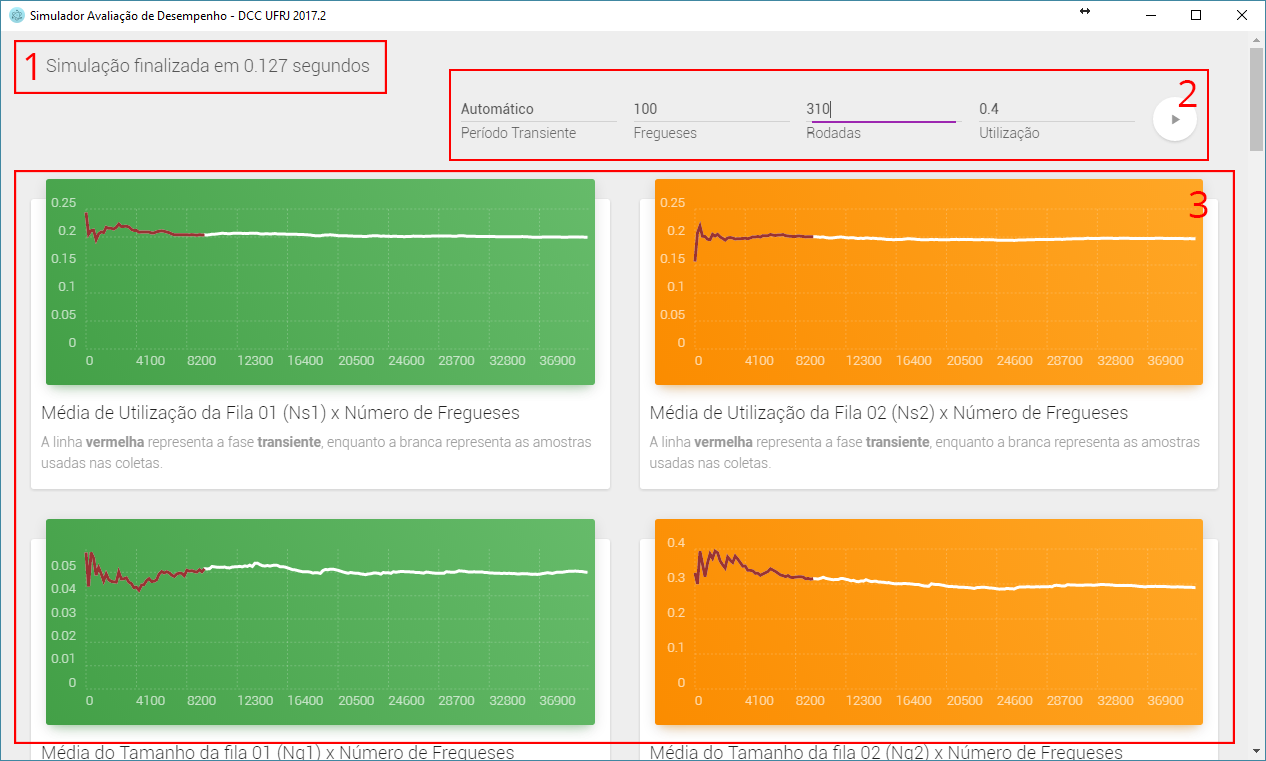
\includegraphics[width=1\textwidth]{./graficos/instructions/SimADViewInst.png}
\vspace{-15mm}
\end{figure}

\begin{enumerate}
	\itemsep1em
	\item \textbf{Status}: nesta área é possível acompanhar o tempo de execução da última simulação.
	\item \textbf{Parâmetros}: nesta área é possível alterar os parâmetros ou deixar os valores pré-definidos. Fase Transiente \emph{Automática} significa que ela vai ser definida em função de $\rho$, com os valores discutidos na seção 3. Para rodar uma nova simulação, preencha os parâmetros e clique em no botão \emph{Play}.
	\item \textbf{Gráficos}: Os gráficos verdes pertencem à fila 1, enquanto os gráficos laranjas pertencem à fila 2. A linha vermelha representa a fase transiente, e a branca representa as rodadas, de onde as métricas foram coletadas.

\begin{figure}[H]
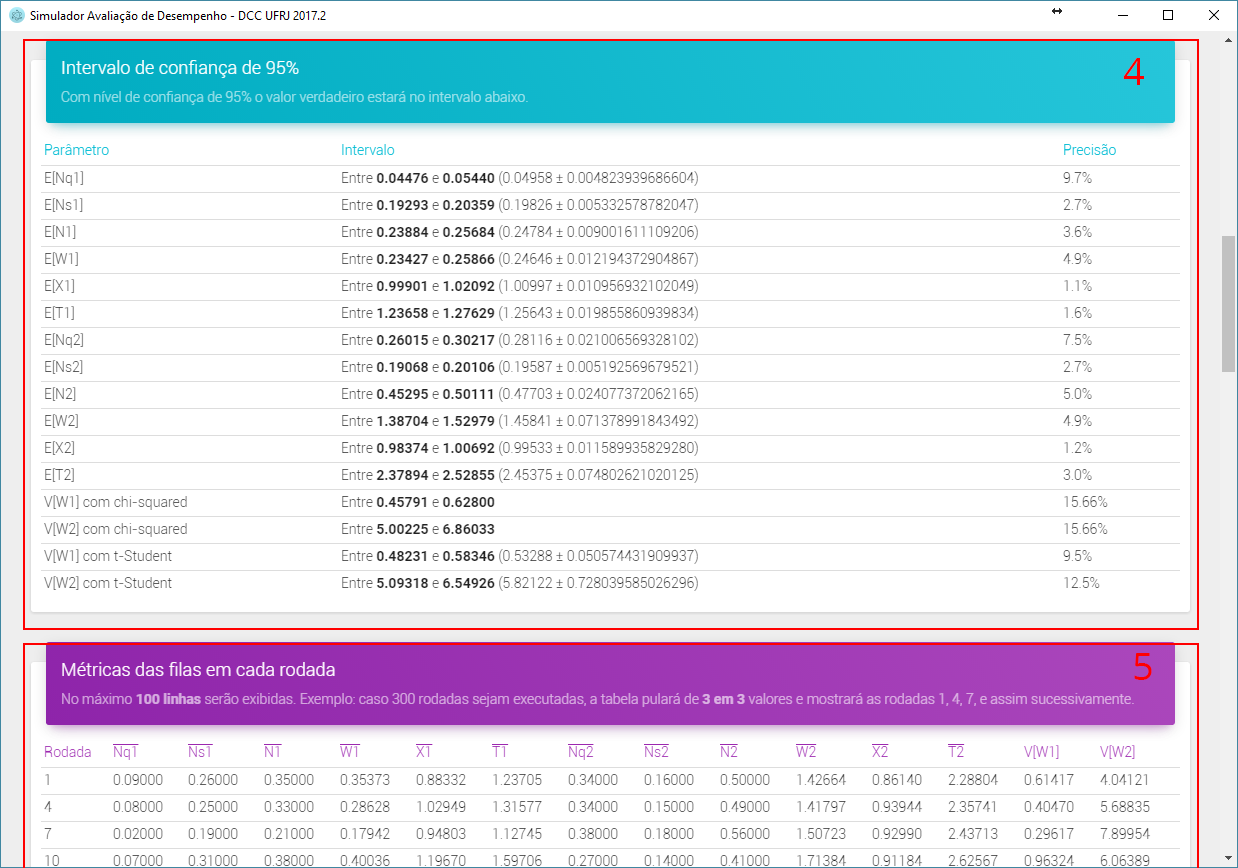
\includegraphics[width=1\textwidth]{./graficos/instructions/TablesAD.png}
\vspace{-10mm}
\end{figure}

	\itemsep1em
	\item \textbf{Tabela do IC}: nesta tabela é possível visualizar o intervalo de confiança de 95\% e a precisão de todas as métricas do sistema.
	\item \textbf{Métricas da Rodada}: nesta tabela é possível visualizar as médias amostrais de cada rodada, e a média de todas as rodadas, na última linha. Para impedir que esta tabela fique muito extensa, caso o número de rodadas seja maior que 100, algumas rodadas não serão exibidas na tabela.

\vspace{5mm}
\begin{figure}[H]
\begin{center}
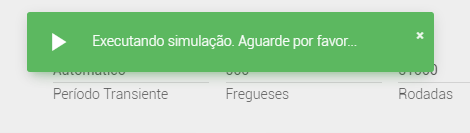
\includegraphics[width=0.8\textwidth]{./graficos/instructions/executando.png}
\end{center}
\vspace{-5mm}
\end{figure}

	\item \textbf{Notificação de Execução}: esta notificação avisa que a simulação está em execução. Enquanto a simulação roda, a interface gráfica fica bloqueada até que a simulação termine.

\vspace{5mm}

\begin{figure}[H]
\begin{center}
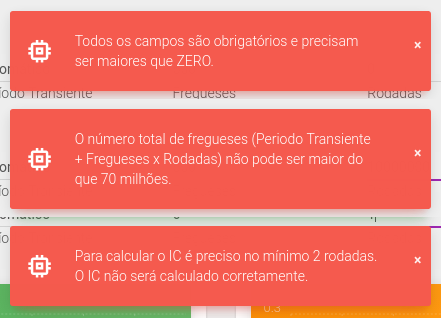
\includegraphics[width=0.8\textwidth]{./graficos/instructions/erros.png}
\end{center}
\vspace{-5mm}
\end{figure}

	\item \textbf{Notificações de Erro}: caso algum parâmetro tenha um valor inválido, serão exibidas notificações explicando o motivo do erro.
	
	\item \textbf{Dúvidas ou Problemas}: caso algum problema para rodar o simulador seja encontrado ou alguma dúvida precise ser esclarecida, basta entrar em contato com algum integrante do grupo.
	
\end{enumerate}
\end{document}